\documentclass[10pt,a4paper]{article}
\usepackage[utf8]{inputenc}
\usepackage{amsmath}
\usepackage{amsfonts}
\usepackage{amssymb}
\usepackage{listings}
\usepackage{graphicx}

\usepackage{color}

\def\File#1{\textsf{#1}}
\def\Code#1{\texttt{#1}}
\def\Key#1{\textsf{#1}}

\definecolor{mygreen}{rgb}{0,0.6,0}
\definecolor{mygray}{rgb}{0.5,0.5,0.5}
\definecolor{mymauve}{rgb}{0.58,0,0.82}

\lstset{ %
  backgroundcolor=\color{white},   % choose the background color; you must add \usepackage{color} or \usepackage{xcolor}
  basicstyle=\footnotesize,        % the size of the fonts that are used for the code
  breakatwhitespace=false,         % sets if automatic breaks should only happen at whitespace
  breaklines=true,                 % sets automatic line breaking
  captionpos=b,                    % sets the caption-position to bottom
  commentstyle=\color{mygreen},    % comment style
  deletekeywords={...},            % if you want to delete keywords from the given language
  escapeinside={\%*}{*)},          % if you want to add LaTeX within your code
  extendedchars=true,              % lets you use non-ASCII characters; for 8-bits encodings only, does not work with UTF-8
  frame=single,                    % adds a frame around the code
  keywordstyle=\color{blue},       % keyword style
  language=Octave,                 % the language of the code
  morekeywords={*,...},            % if you want to add more keywords to the set
  numbers=left,                    % where to put the line-numbers; possible values are (none, left, right)
  numbersep=5pt,                   % how far the line-numbers are from the code
  numberstyle=\tiny\color{mygray}, % the style that is used for the line-numbers
  rulecolor=\color{mygray},         % if not set, the frame-color may be changed on line-breaks within not-black text (e.g. comments (green here))
  showspaces=false,                % show spaces everywhere adding particular underscores; it overrides 'showstringspaces'
  showstringspaces=false,          % underline spaces within strings only
  showtabs=false,                  % show tabs within strings adding particular underscores
  stepnumber=2,                    % the step between two line-numbers. If it's 1, each line will be numbered
  stringstyle=\color{mymauve},     % string literal style
  tabsize=2                       % sets default tabsize to 2 spaces
%  title=\lstname                   % show the filename of files included with \lstinputlisting; also try caption instead of title
}

\title{01435 Practical Cryptanalysis}
%\author{Kim Rostgaard Christensen - s084283}
\author{Thomas Pedersen - s103665}
\begin{document}
\maketitle

\paragraph*{Exercise 15} For $m = $ values, we get the following plot.
\begin{figure}[h]
\centering
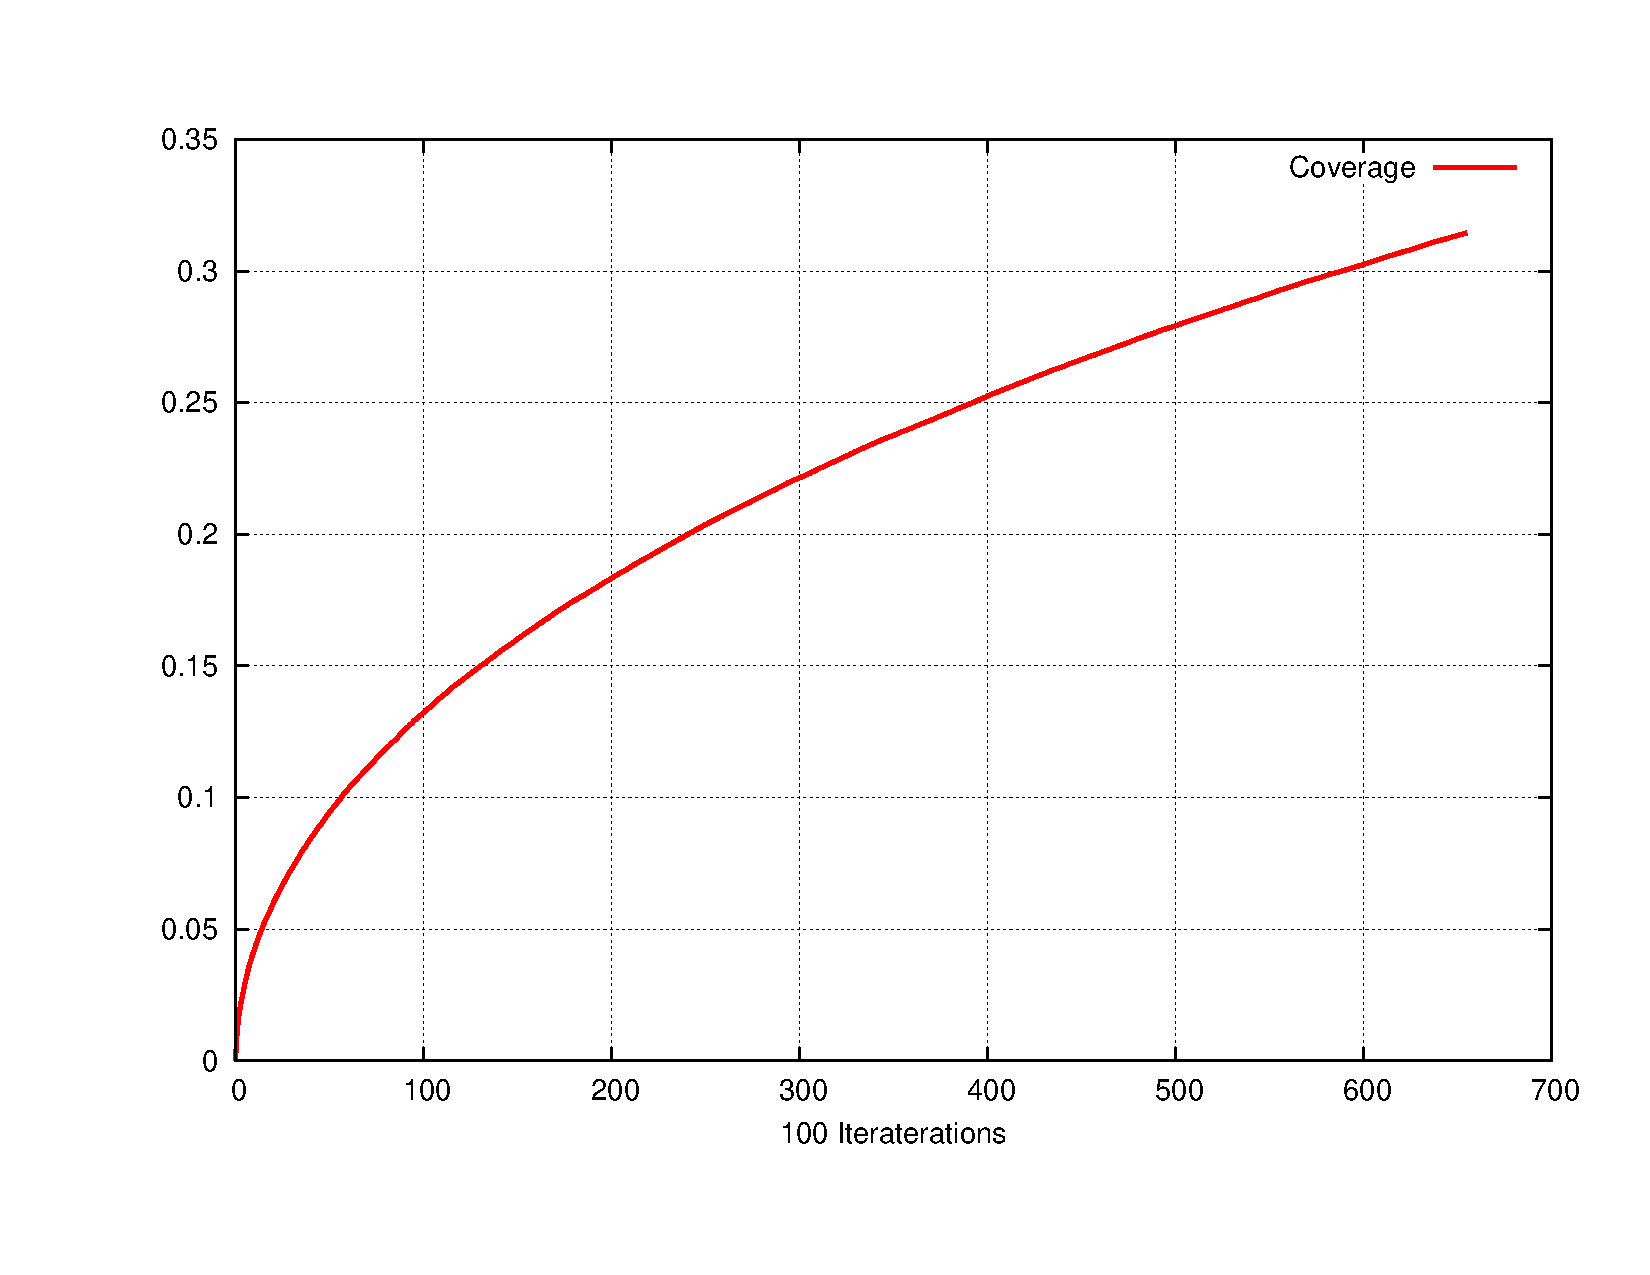
\includegraphics[scale=0.4]{../output/ex15.pdf}
 \caption{Data plot}
 \label{fig:ex15}
\end{figure}
Given the democratic voting in class, this graph fits nicely the assumption that coverage is around ~30%.

\paragraph*{Exercise 16}

\paragraph*{Exercise 17}
\begin{figure}[h]
\centering
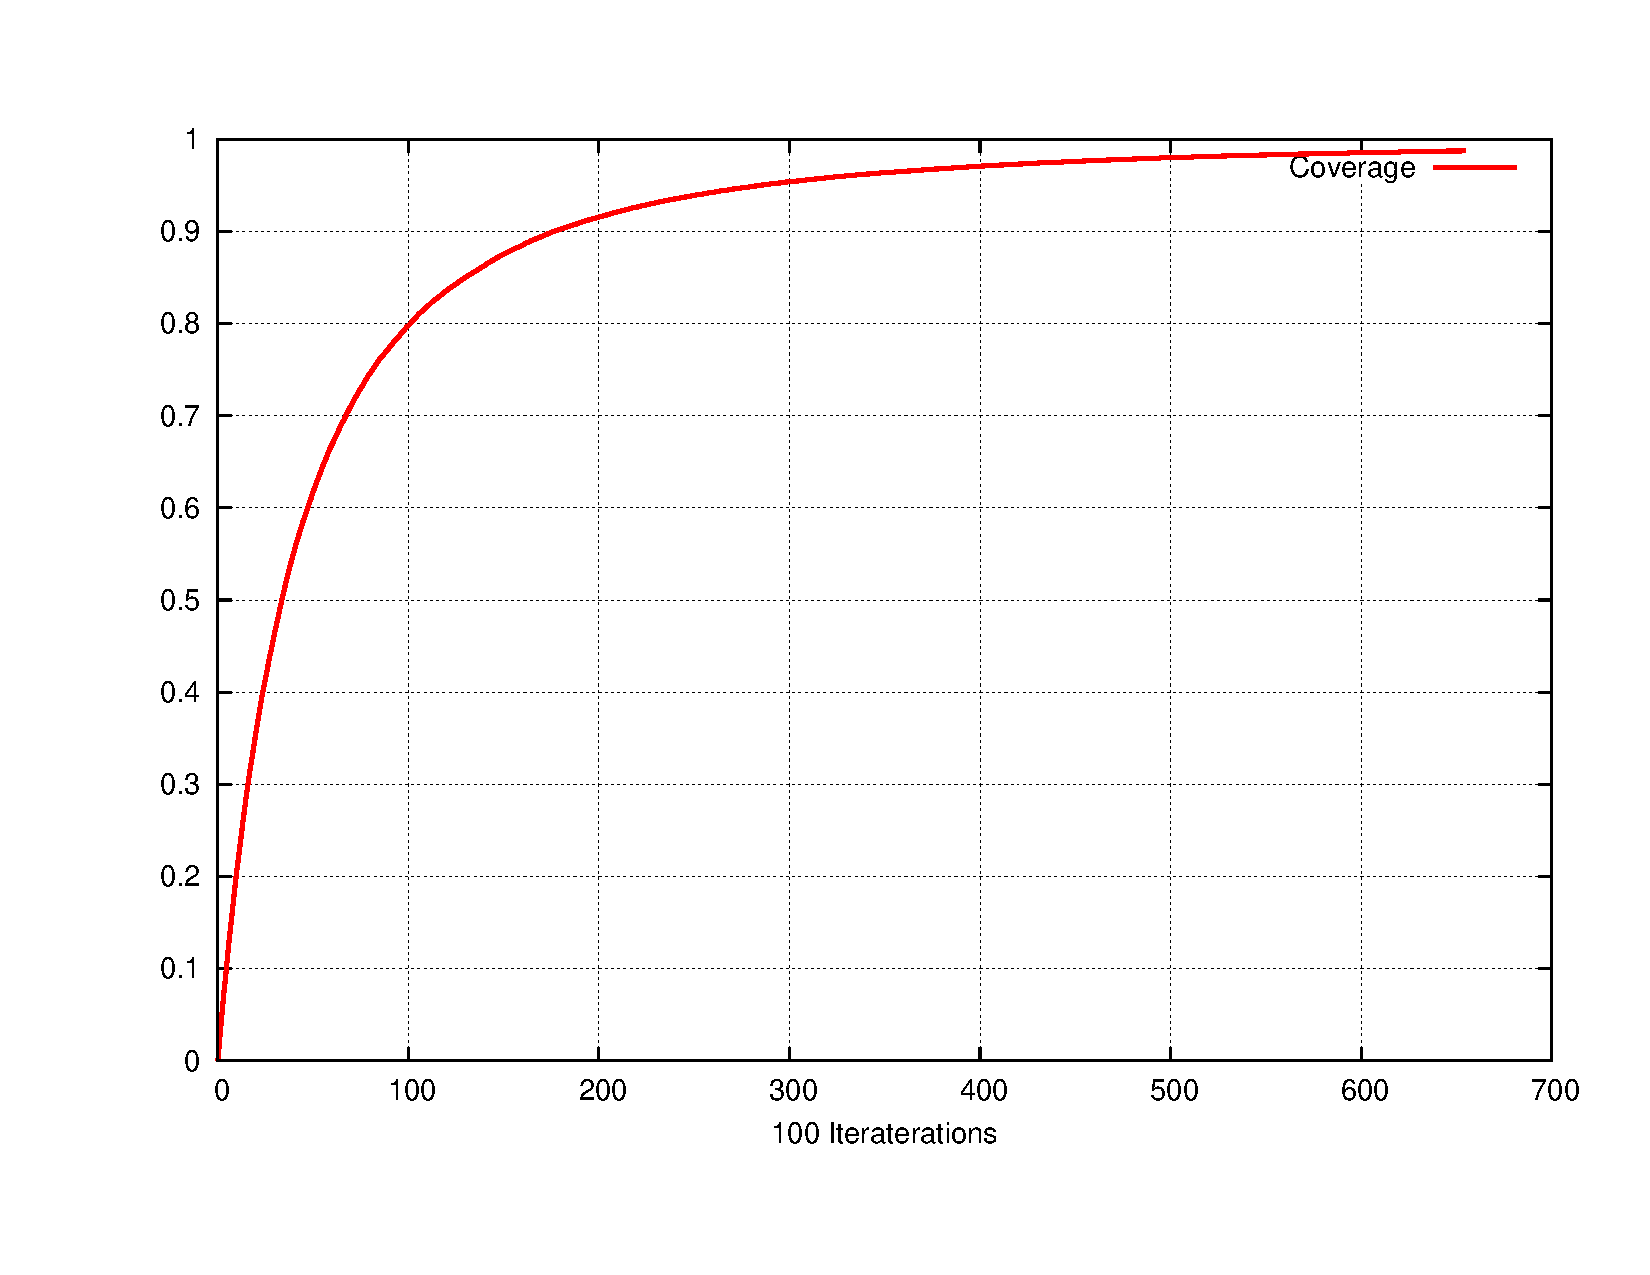
\includegraphics[scale=0.4]{../output/ex17.pdf}
 \caption{Data plot}
 \label{fig:ex17}
\end{figure}

\begin{figure}[h]
\centering
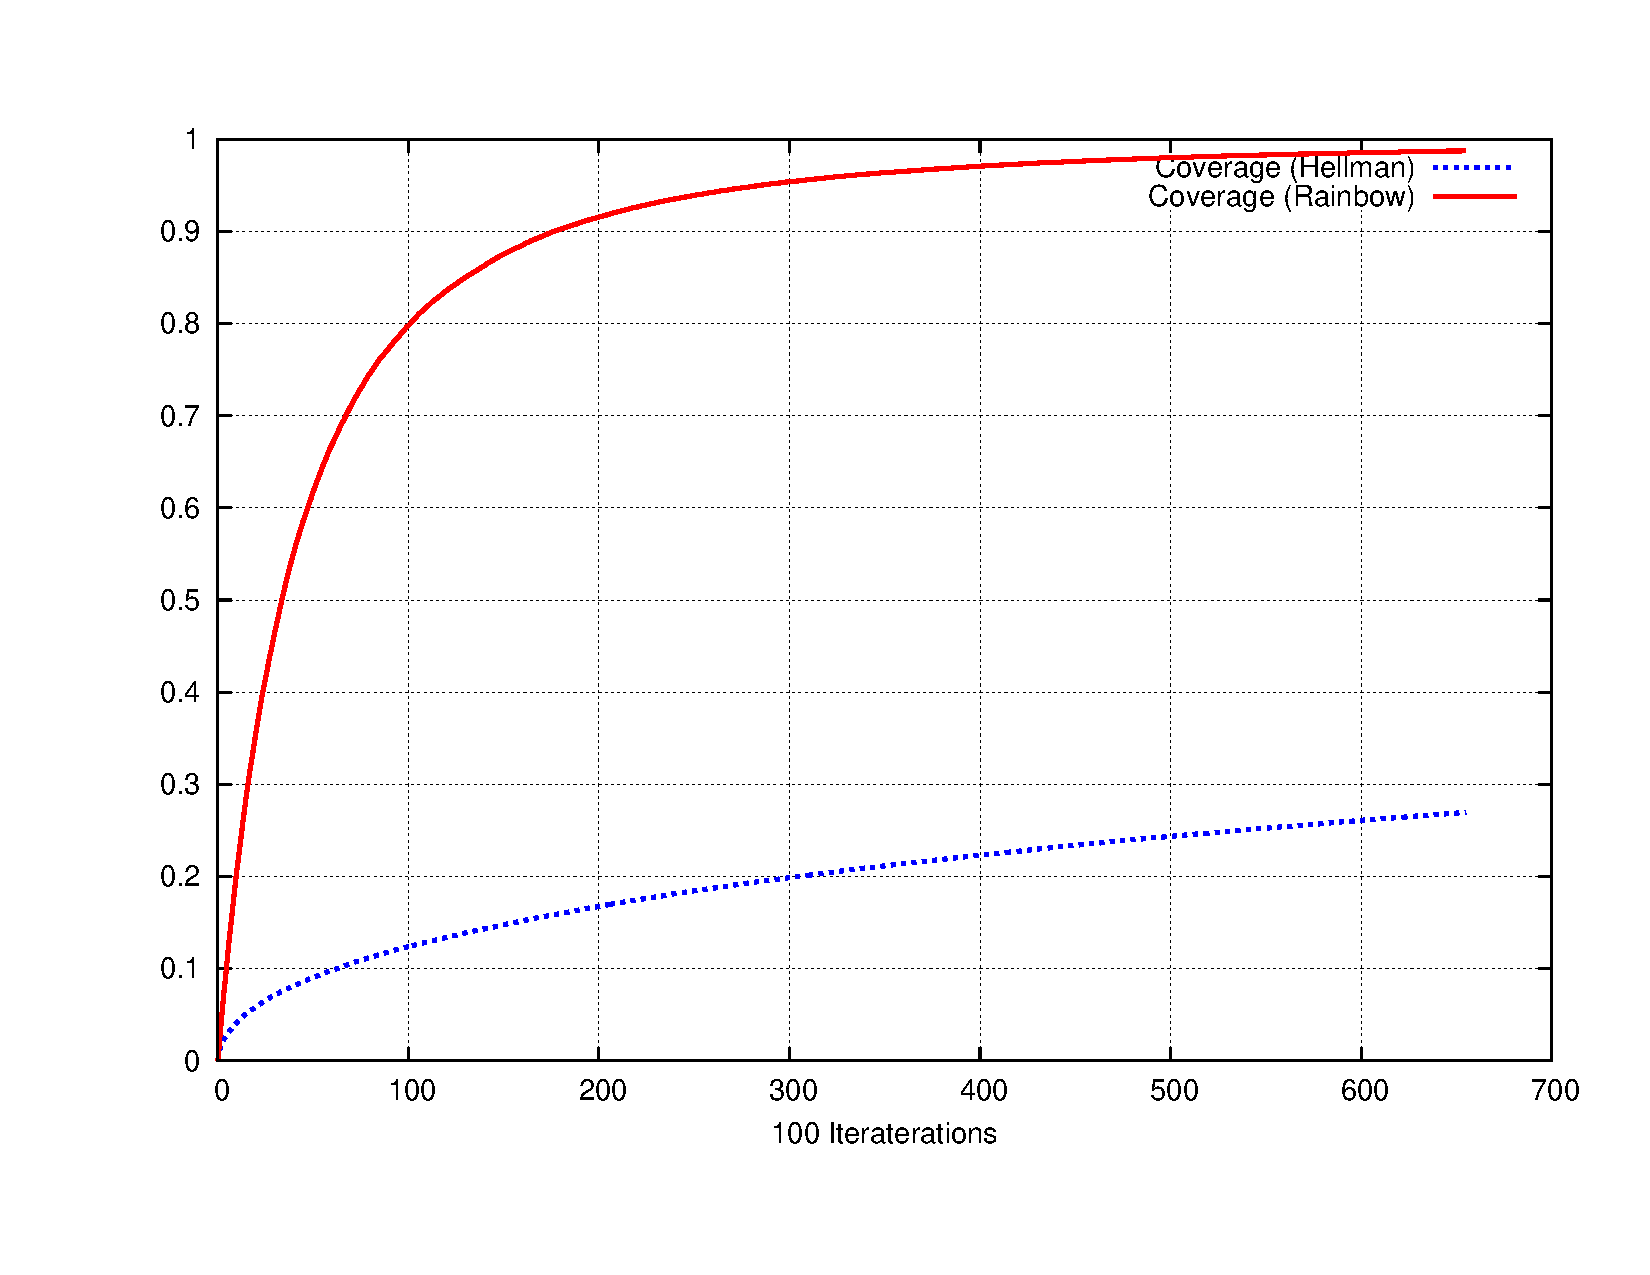
\includegraphics[scale=0.4]{../output/ex17a.pdf}
 \caption{Data plot}
 \label{fig:ex17a}
\end{figure}

\end{document}